\chapter{Pose estimation I: Using a fixed camera}

The policy trained in simulation for pushing a cube to some goal position was
shown to work on the real robotic system with only some minor tweaks.  To know
where the cube was positioned, a LIDAR was used.  Using the LIDAR for pose
estimation of the cube however required that no other objects were accidentally
measured, and used the fact that the position of the cube can be described by a
bounded line in the plane. A more general approach is to infer the pose from a
camera. A usual setup in robotics is to have a camera at a fixed position and
infer poses under the assumption that the camera does not shift position.
Experiments are here first described for estimation under this assumption and
then extended for estimation from a non-fixed camera.

\section{Method}

A camera was mounted at a fixed position as shown in figure
\ref{fig:camera_placement_fixed}. A LIDAR was used to label the pose of the
cube in the coordinate frame of the robot. In total, 10'000 RGB images were
collected during execution of the trained policy. For each picture, depth
channel data was also collected to evaluate the difference in performance when
adding this information. For the depth channel, the camera returns numbers in
the range $[0, 255]$ aligned for each pixel in the color image. The distance
$0$ is in practice never registered but used to represent that depth for this
pixel is missing.

\begin{figure}[h!]
    \centering
    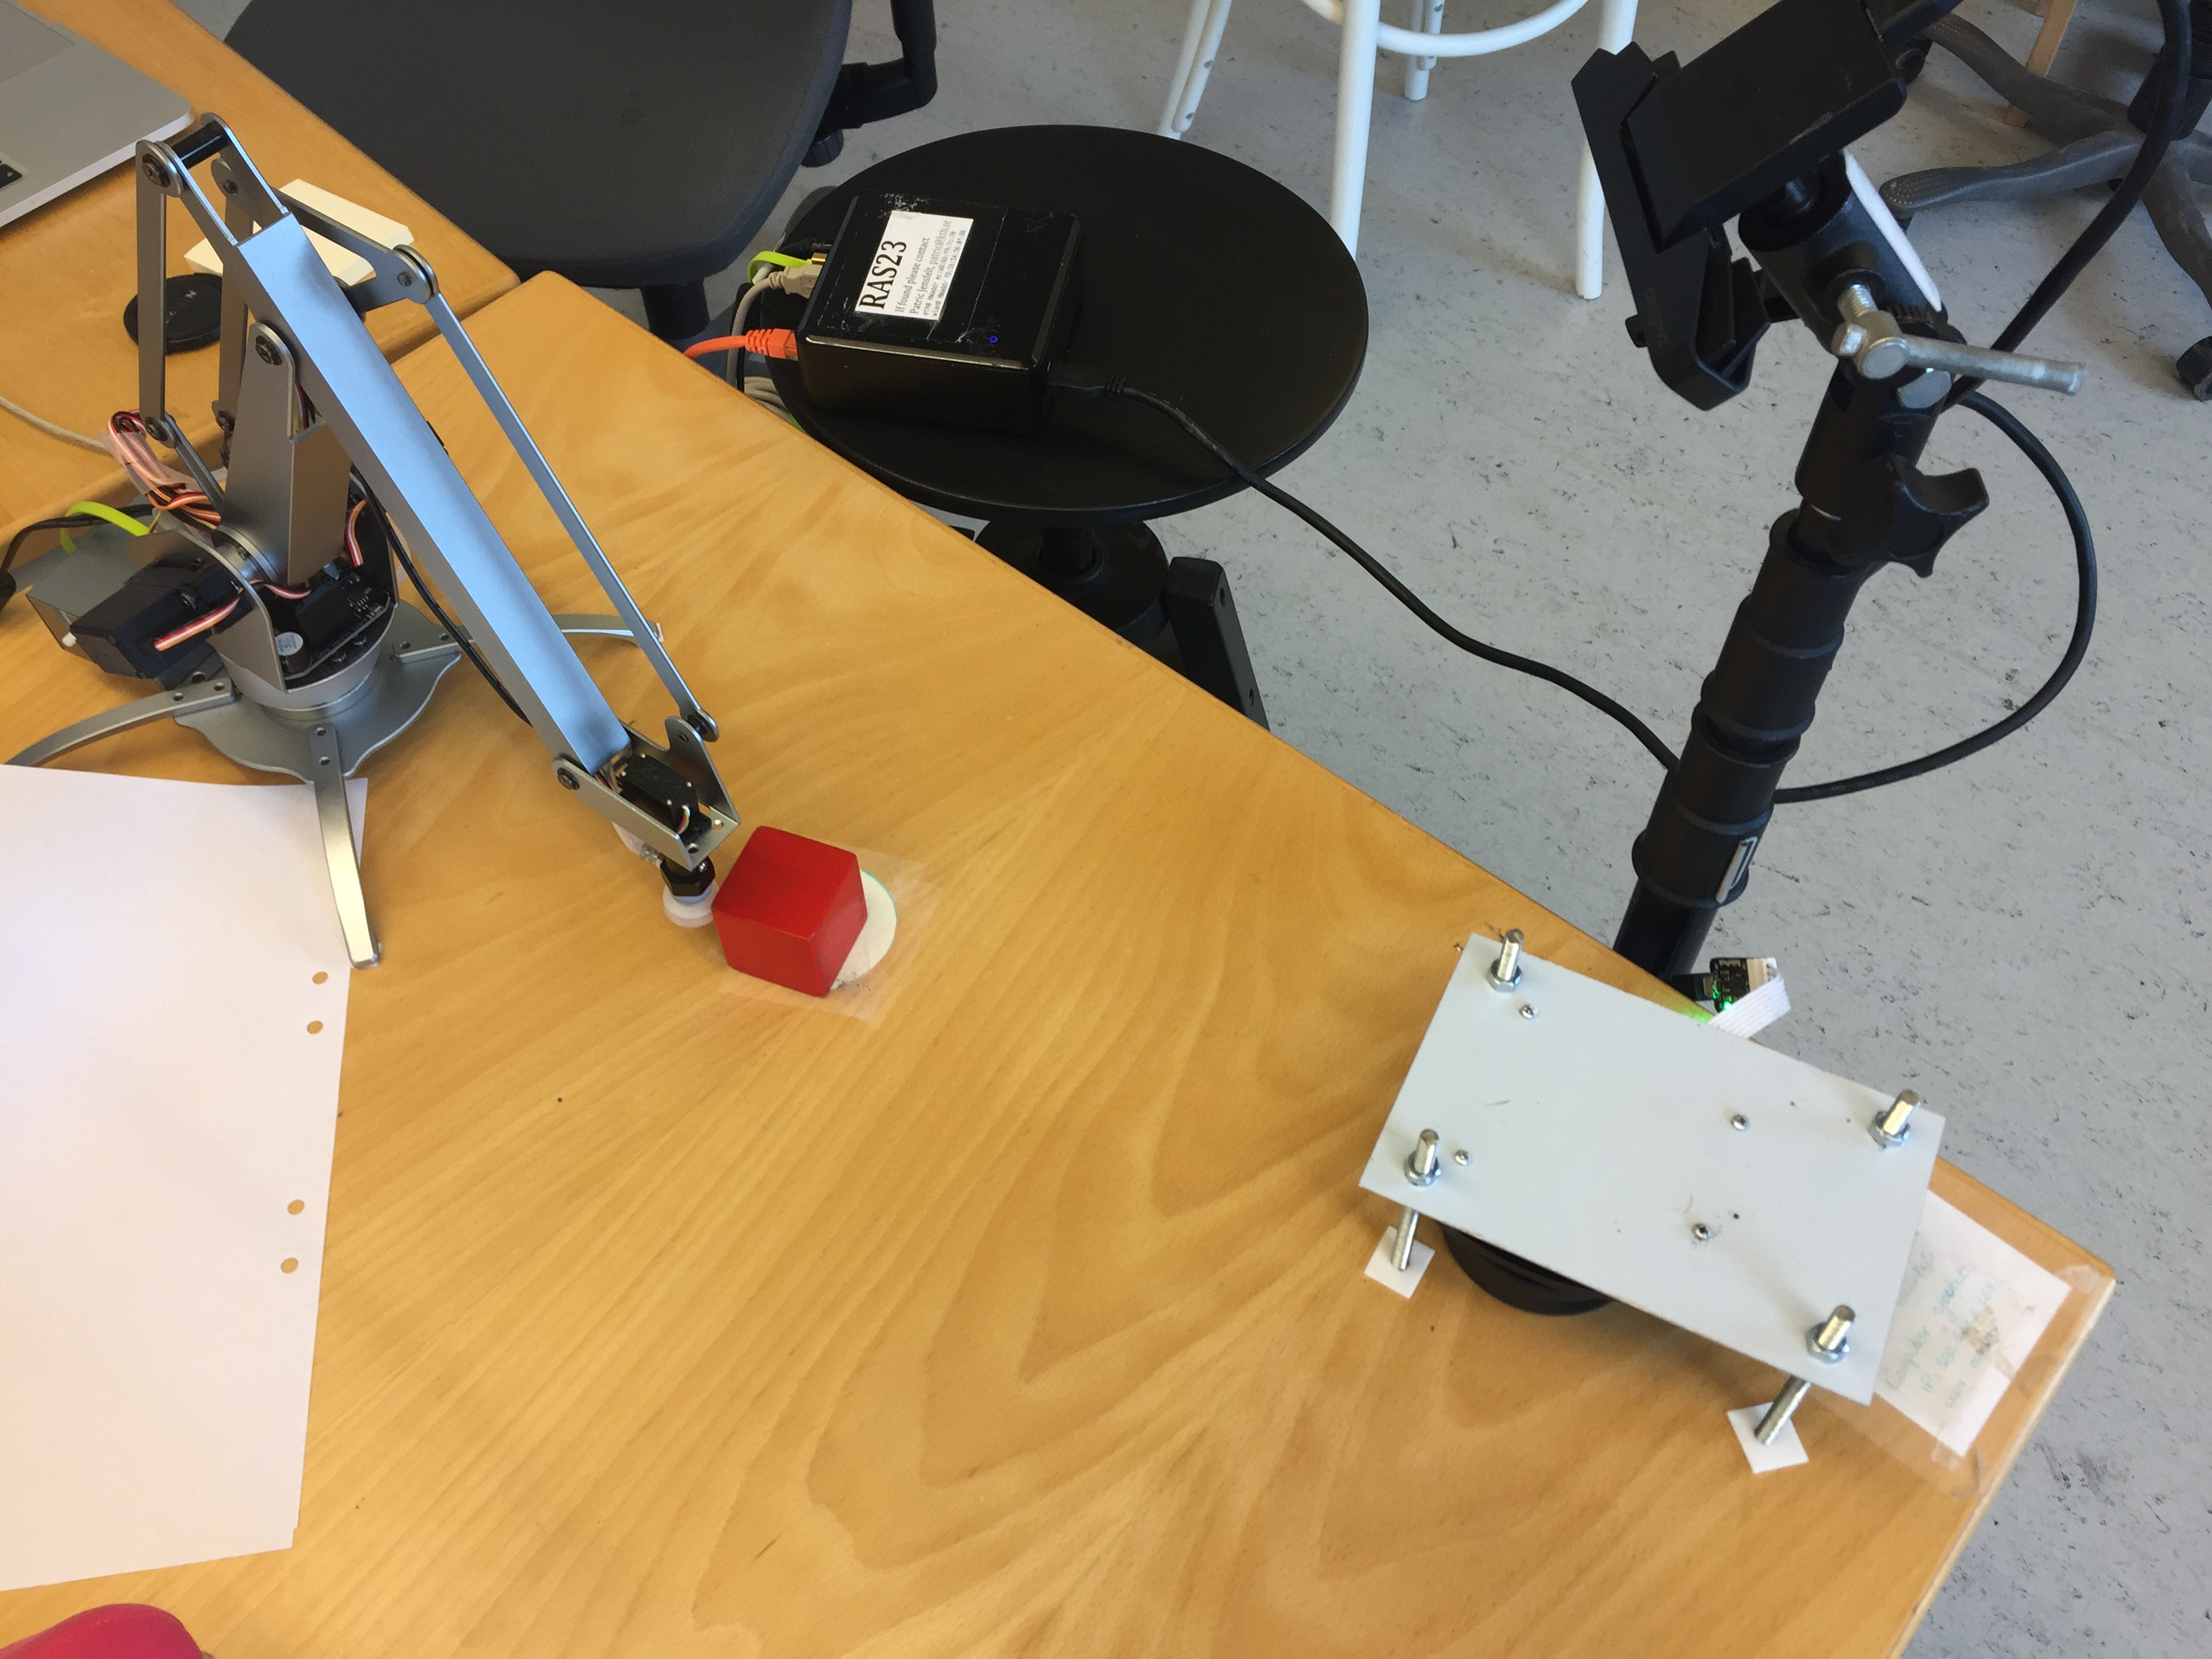
\includegraphics[width=0.4 \textwidth]{res/camera_placement_fixed.jpg}

    \caption{Fixed camera placement for pose estimation of the cube.}

    \label{fig:camera_placement_fixed}
    
\end{figure}

The first part of the network in figure \ref{fig:gps_net} was used, with two
hidden layers of 100 hidden ELU activated units each after the 2-D expected
position. The output was a 2-dimensional linear layer predicting the cube
position in the robot coordinate frame. For incorporating depth into the
network, I propose a layout, shown in figure \ref{fig:depth_net}, where depth
is input at two locations in the network. The first place is simply as a fourth
dimension into the first convolutional layer. The second place is to append the
expected distance $\mathbb{E}[D_k]$ for each feature $k \in [1, 32]$ to the
fully connected layers, using the spatial softmax as the probability when
calculating the expectation:

\begin{figure}[h!]
    \centering
    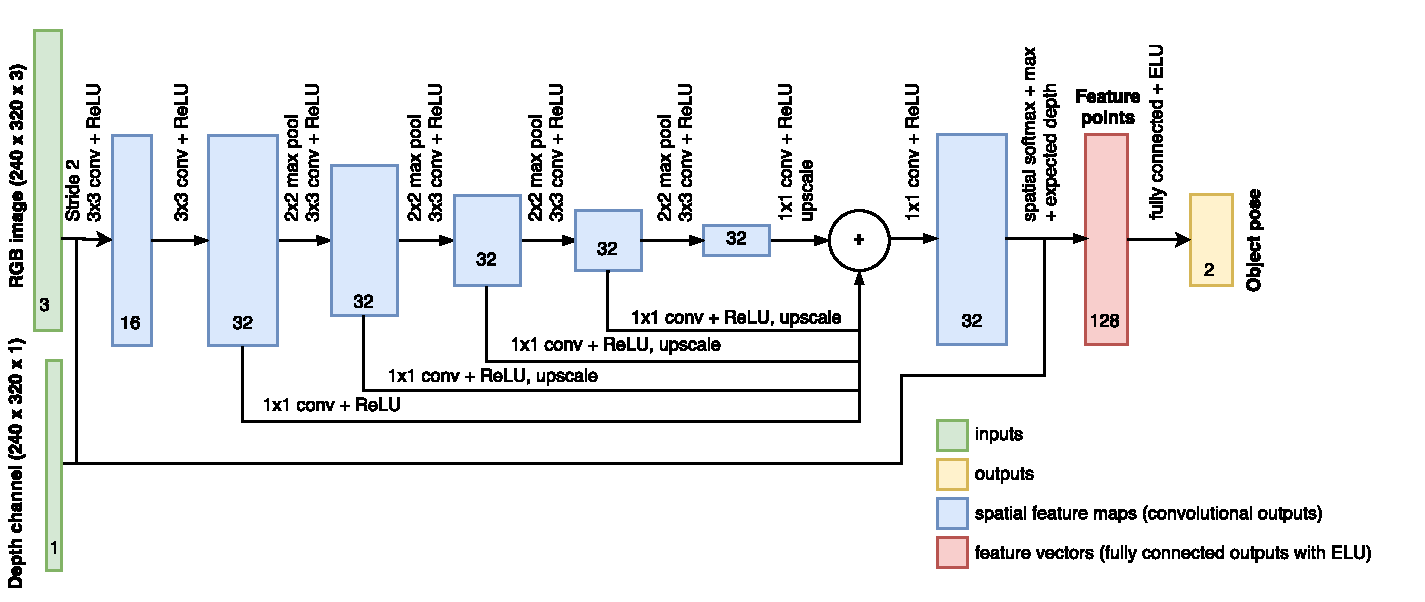
\includegraphics[width=1.0 \textwidth]{res/depth_net.pdf}

    \caption{Proposed pose estimation network incorporating depth information.
    Input to the first convolutional layer is a 4-channel RGBD image. Using the
    spatial softmax as a per-feature probability distribution, expected depths
    per feature map are also concatenated with the expectation over image
    coordinates. As a measure of uncertainty in each feature, the maximum
    activation for each feature map, after the spatial softmax, are also
    concatenated with the input to the fully connected layer.}

    \label{fig:depth_net}
    
\end{figure}

\begin{equation}
    \mathbb{E}[D_{k}] = \sum_{i, j} p(c_{i, j, k}) d_{i, j}
\end{equation}

Here, $p(c_{i, j, k})$ is the output of the spatial softmax at pixel $(i, j)$
for feature map $k$ and $d_{i, j}$ the registered depth at pixel $(i, j)$. The
network was trained by minimizing the mean square error and using the Adam
optimizer. The training and validation losses are plotted in figure
\ref{fig:depth-vs-rgb} showing that only using RGB converges faster and that
adding depth did not contribute to better scores in this experiment.

\begin{figure}[h!]
    \centering
    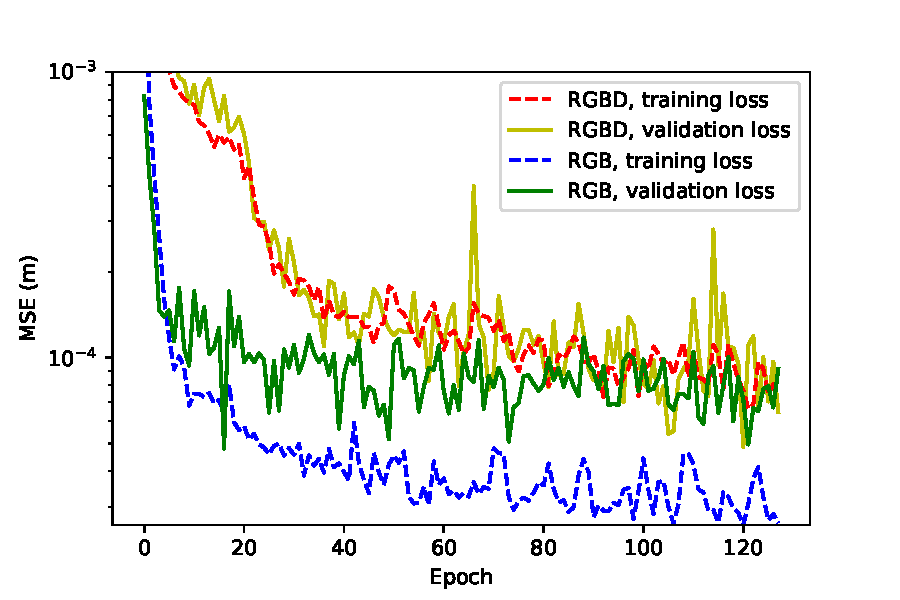
\includegraphics[width=0.6 \textwidth]{res/depth-vs-rgb.pdf}

    \caption{Training curves for pose estimation from a fixed position camera.
    Adding depth information did not lower training scores, only slowing down
    the time needed to converge.}

    \label{fig:depth-vs-rgb}
    
\end{figure}

\section{Results \& Discussion}

The trained network using RGB was used instead of the pose estimates from the
LIDAR and tested on a robot. The network needed significantly more time to
evaluate than when using the LIDAR estimates, the algorithm now running at 1-2
Hz compared to approximately at 10Hz using LIDAR estimates. The bottleneck when
using LIDAR estimates are not the actual LIDAR, but rather controlling the
robot and measuring servo angles etc. A video was recorded of the result and
can be seen here: \url{https://youtu.be/vakM-xvhEmE}. A dark gray cup was added
into the workspace without previous tests during recording of the video showing
that the estimation could handle some distraction. Further tests showed that
any red object will disturb the pose estimates, making the policy unsuccessful
in pushing the cube. This was expected though since no distractors were added
during data collection.
